\chapter{Evaluation}
\label{ch:evaluation}

\section{External-Model Study and Harness Correction}

After correction, executable evidence improved one of 23 eligible predictions and caused no regressions, an observed gain of
4.35 percentage points. Related and unrelated passing evidence produced identical binary decisions. The corrected result
leaves a useful benefit unresolved and provides no evidence that this tracker recognised the relevance of a passing check.

The original sealed analysis suggested a 30.43 percentage-point advantage over dialogue alone. Its paired interval was wide
and the exact McNemar comparison was not significant. A full replay then found that the test harness had compared equivalent
sequence values incorrectly. Nineteen of 48 execution records changed:
12 evidence labels and five criterion labels changed, one further criterion record changed its test counts while remaining
unsuccessful, and one missing criterion was reclassified from sandbox error to invalid submission. Thus, 17 binary labels
changed. The count of 19 also includes a test-count change and a failure-status correction.

The corrected 95\% paired case-bootstrap interval was 0.00 to 13.04 percentage points, and the two-sided exact McNemar
test gave $p=1.0$. Only one case had different correctness outcomes between the conditions: evidence corrected that prediction,
while 18 cases were correct under both conditions and four were incorrect under both. The original exact comparison gave
$p=0.0923$. Neither result establishes equivalence. In particular, the corrected interval still includes the declared
ten-percentage-point threshold for a practically meaningful improvement, although the point estimate falls below it.
The experiment therefore leaves a meaningful benefit unresolved. It cannot show that probing has no useful effect.
These intervals describe resampling this small authored corpus and do not account for its shared concept families or a fresh
model run. Figure~\ref{fig:harness-correction} shows how the correction changed the estimated advantage and its interval.

Here, performance means passing the authored criterion checks. Repairing the sequence comparison did not establish that those
checks covered every task requirement. The worked example retains a known coverage limitation: checking returned values did not
establish that the supplied list was changed. The corrected analysis remains a comparison against this limited instrument.

\begin{figure}[tb]
  \centering
  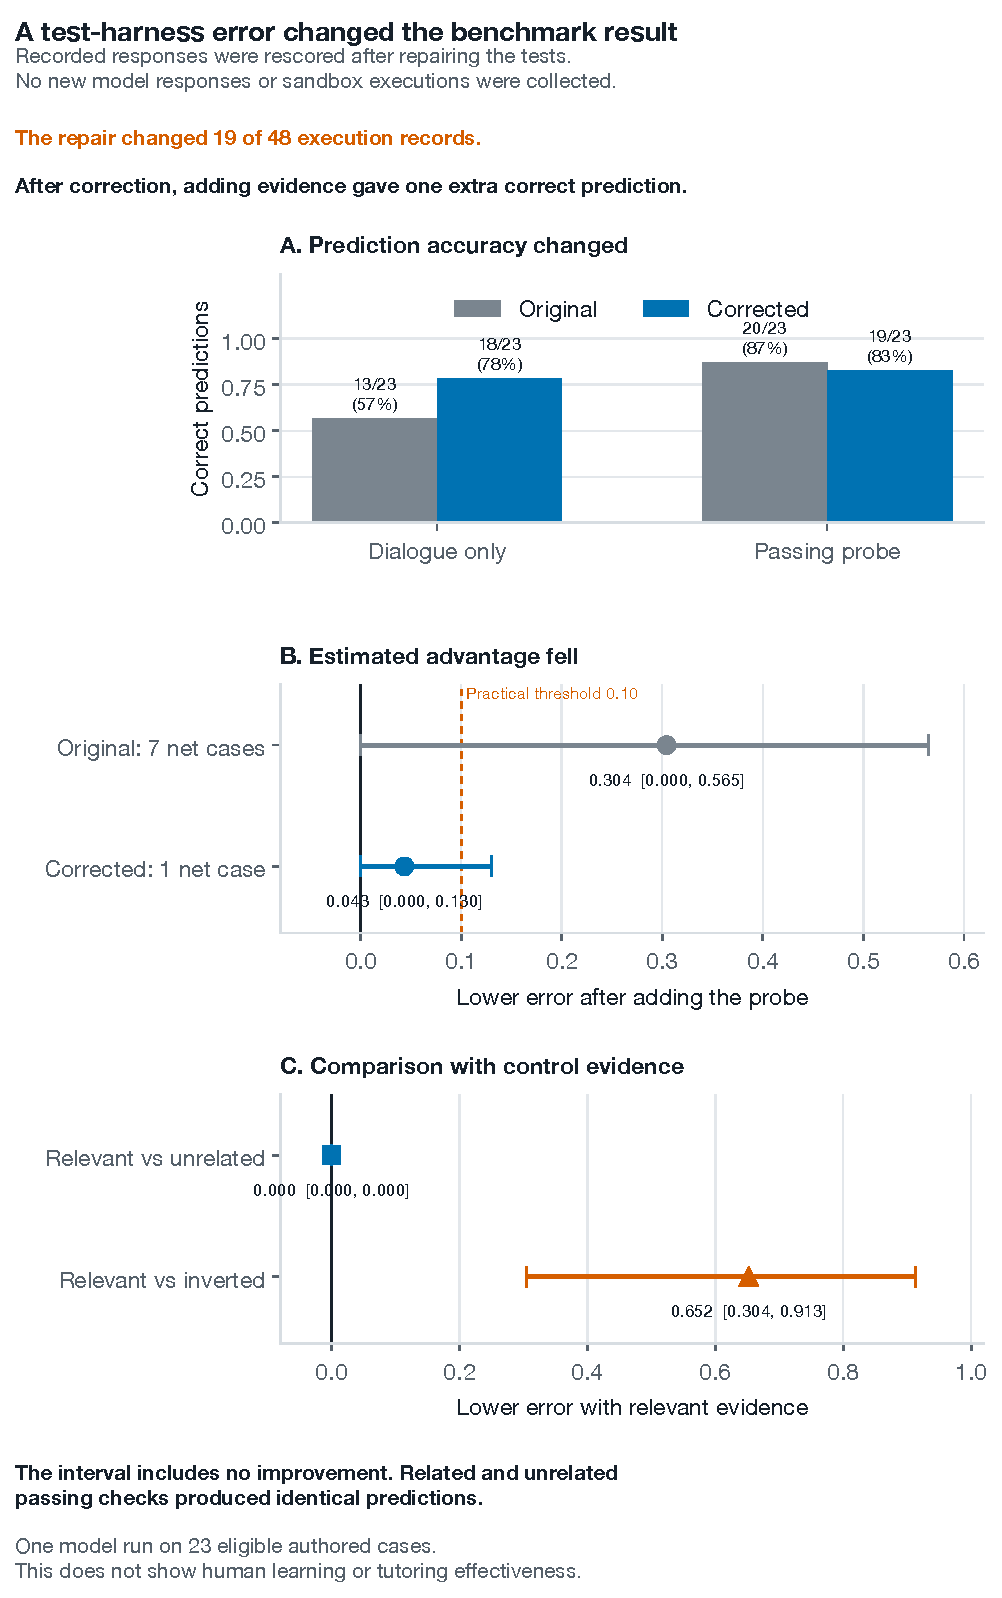
\includegraphics[width=\textwidth,height=0.82\textheight,keepaspectratio]{assets/figures/ch06-evaluation/harness_correction_result.pdf}
  \caption{Effect of correcting the test harness on 23 eligible authored cases. Adding executable evidence to the dialogue
  increased correct predictions from 13/23 to 20/23 under the original scoring, and from 18/23 to 19/23 after correction.
  The corrected reduction in classification error was 4.3 percentage points (95\% paired bootstrap interval: 0 to 13.0).
  Positive differences favour adding evidence. Related and unrelated passing checks produced identical predictions.
  The correction reuses one recorded run. It does not measure learning.}
  \label{fig:harness-correction}
\end{figure}

\subsection{The Missing Criterion Outcome}

Case \texttt{h-c2m2-03} has no valid binary criterion outcome. The original execution was recorded as a sandbox error.
The corrected replay records an invalid submission. Neither status is an observed test failure, so the case remains excluded
from the 23-case primary analysis.

Its saved dialogue-only and valid-evidence predictions both indicate success. If a valid criterion outcome had been failure,
both would be wrong. If it had been success, both would be right. Holding the saved predictions and all other outcomes fixed,
the two hypothetical completions give 18/24 versus 19/24 correct predictions, or 19/24 versus 20/24. In either case, the
valid-evidence advantage would be $1/24$, or 4.17 percentage points. The missing case cannot add a disagreement between these
two conditions under either binary completion. Their observed advantage remains $1/23$, or 4.35 points.

This is a descriptive sensitivity calculation, not an imputed observation or a new primary analysis. It does not justify
treating invalid submissions as failures, assuming that missingness is random, or extending the finding beyond the authored
cases. The corrupted-evidence prediction for this case is failure, so the same cancellation does not apply to every secondary
comparison. The small corpus, shared concepts and single model run remain separate limitations.

For the secondary comparisons, valid and unrelated evidence have identical predictions on all 24 cases, including the missing
case. Their difference therefore remains zero under either binary completion. Valid evidence exceeds corrupted evidence by a
net 15 correct predictions among the 23 observed cases. Adding a hypothetical failure for the missing case reduces that net
difference to 14. Adding a success increases it to 16. Across 24 cases, these alternatives give advantages of 58.33 and
66.67 percentage points, respectively (the observed 23-case difference is 65.22 points).

The frozen combined control contrast averages the valid-versus-unrelated and valid-versus-corrupted differences. Its observed
value is 32.61 percentage points. The two hypothetical completions give 29.17 and 33.33 points. These describe alternative
completions of the missing outcome. The positive combined contrast comes entirely from the corrupted-evidence comparison.
It cannot establish that relevant evidence helps more than unrelated evidence. No secondary outcome is filled in, and the
frozen analyses retain their original 23-case denominator.

\subsection{Reviewer Agreement and Its Limits}

The two public-answer reviewers agreed on all 24 cases. Both assigned 23 answers to the correct category and one to the
conflicting category. No disagreement required adjudication. Raw agreement and unweighted Cohen's kappa were both 1.0.
These ratings concern the visible answers, not the later criterion outcomes. With four of the six categories unused, this
sample provides little evidence about how consistently the reviewers would distinguish the full category set.

The separate failure review covered six records, assessed by the author and an independent reviewer. Both final submissions assigned four to item ambiguity or test defect and
two to no observed failure. Raw agreement and kappa were again 1.0, with no adjudication required. These six records are a
selected diagnostic set, not a random sample of all possible failures. Their category counts cannot estimate a general failure
rate or establish that every relevant defect was found.

The archived author sheet contains an earlier version with three different categories. The agreement calculation uses the
revised author sheet and the final independent submission. It therefore describes agreement after revision. It does not
establish agreement between initial judgements or show whether the revision process affected their convergence.

Agreement shows that the submitted categories matched. It does not prove that they were correct, that test coverage was complete,
or that the chosen category identifies a unique cause. A shared taxonomy can encourage a shared interpretation. The reliability
reports summarise final submissions. Preserved review records are needed to inspect their revision
history. The complete harness correction remains separate execution evidence and must not be inferred from agreement alone.

\subsection{Recorded Workload and Missing Measurements}

The original external run recorded 72 Cerebras responses: 48 across the public-answer and evidence channels, followed by
24 criterion responses. Their total usage was 15,899 input tokens and 16,684 output tokens. Summed provider latency was
32.70 seconds. This is the sum of individual recorded request latencies, not elapsed experiment time or the waiting time of a
student using the tutor. Response-capture spans were about 633 seconds for decision generation and 364 seconds for criterion
generation, in separate phases.

Of 48 original sandbox execution attempts, 47 completed: all 24 evidence executions and 23 of 24 criterion executions.
The missing criterion left 23 cases eligible for paired analysis. Completion is distinct from passing a test. Subsequent
harness correction reused recorded model responses. It did not constitute another independent model evaluation.

Provider charges were not reported. Sandbox duration, CPU use and memory use were also absent from the original records.
These quantities remain unavailable, rather than being treated as zero. The original reconciliation report also predates the
complete harness correction. Its partial corrected pass/fail tallies are superseded. Only its original workload accounting is
used here.

An evidence-informed condition required the public response plus an additional model response and sandbox execution. Criterion
generation was an evaluation requirement, not an input available to a deployed prediction rule. This accounting establishes
extra experimental work, but not realised financial savings, a minimum-cost selection policy, or faster classroom tutoring.
The probe selection simulator performs no provider or sandbox call, and its probe allocation cannot fill these missing cost measurements.

\FloatBarrier
\section{Bounded Update Study}

Across five adverse simulator conditions, the bounded tracker had mean Brier error 0.0094 lower than ordinary channel-aware Bayes.
The paired 95\% interval was $[-0.0101,-0.0086]$. Under clean evidence, bounding increased Brier error by 0.0033, and the upper
interval bound of 0.0042 remained below the fixed 0.0100 tolerance. Figure~\ref{fig:tracker-result} shows the comparison
across the tested conditions.

The favourable adverse-condition average hides differences between conditions. Bounded updating reduced Brier error under
uninformative, inverted and reliability-misspecified evidence, but increased it under missing and contradictory evidence.
It passed the declared rule for average improvement and the permitted loss under clean evidence. This is
an empirical result, separate from the per-observation bound on log-odds movement.

\begin{figure}[tb]
  \centering
  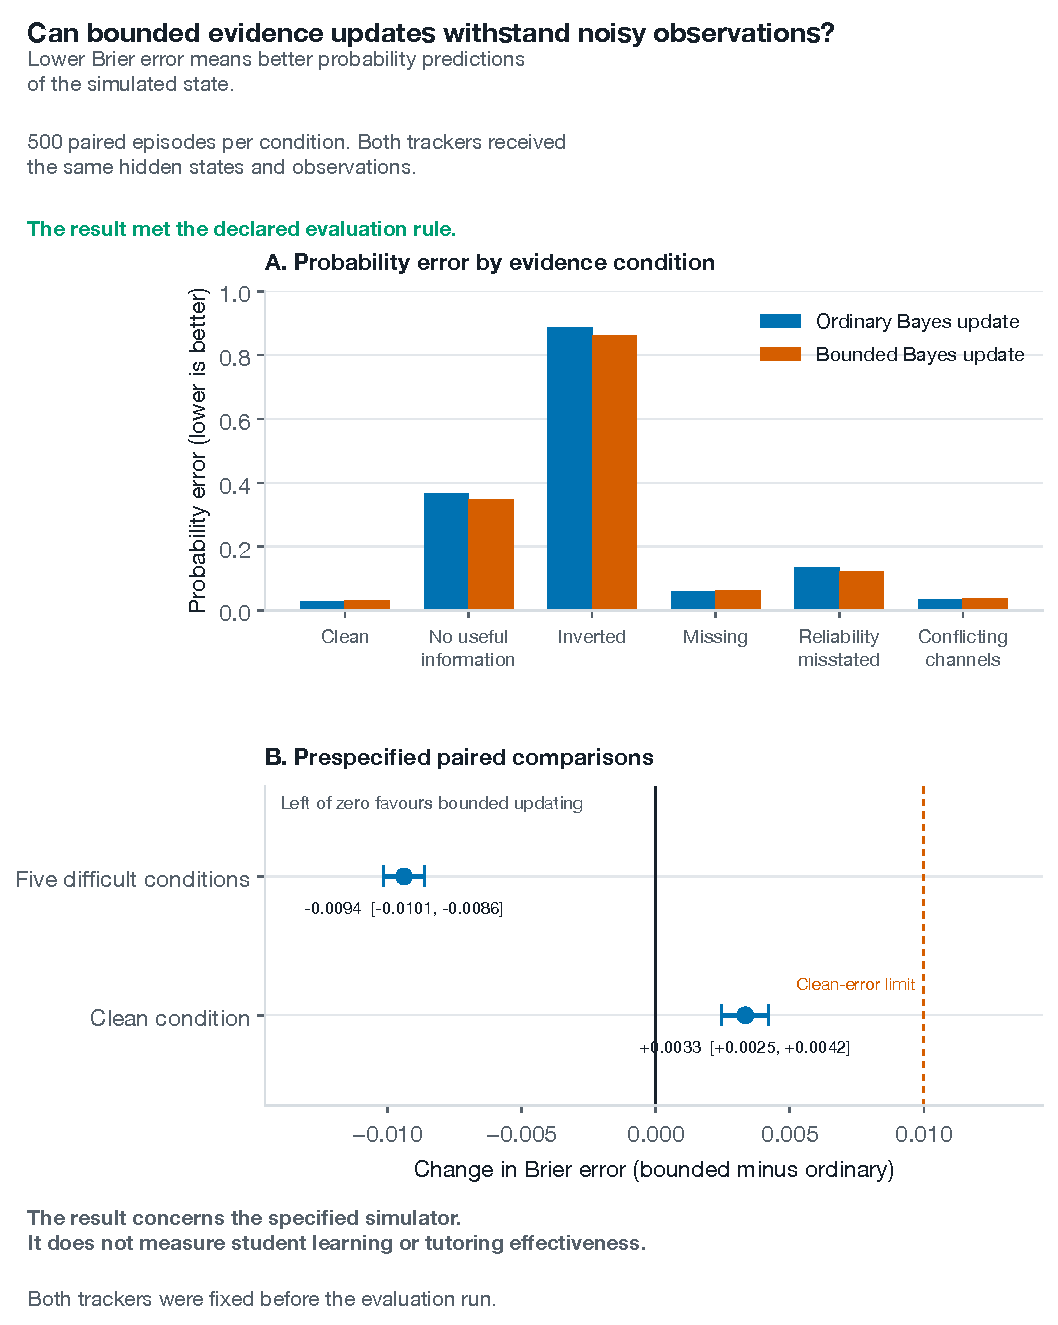
\includegraphics[width=\textwidth,height=0.82\textheight,keepaspectratio]{assets/figures/ch06-evaluation/tracker_study_canonical.pdf}
  \caption{Ordinary and bounded Bayesian updates across 500 matched simulated episodes per condition. Lower Brier error
  indicates better probability predictions. Differences are bounded minus ordinary. Negative values favour bounded updating.
  Paired 95\% intervals describe the equally weighted average across five adverse conditions and the clean condition.
  Bounded updating improved the adverse average, while error increased under missing, contradictory and clean evidence.
  The results concern the specified simulator. They do not measure student learning.}
  \label{fig:tracker-result}
\end{figure}

\FloatBarrier
\section{Selective Acquisition Study}
\suppressfloats[t]

At the fixed 50\% budget, the proposed policy reduced held-out classification error by 1.19 percentage points relative to random
selection. It increased error by 0.855 percentage points (0.86 when rounded to two decimal places) relative to uncertainty-only
selection and by 0.54 points relative to the plug-in
clipped-belief comparator. All three multiplicity-adjusted intervals excluded zero. The proposed policy therefore failed the declared
all-comparator rule.

The budget was compulsory: every selector that could probe selected 20 of the 40 cases. The candidate therefore chose the
allocation, rather than deciding whether an additional check was worth requesting in the first place. The comparison
concerns which cases were checked under this fixed design. Every selector requested the same number of checks.

These are measured errors of the implemented heuristics. As Chapter~\ref{ch:method} explains, the acquisition score is not
generally expected classification-error reduction. The result therefore cannot establish the performance of an exact
value-of-information optimiser. The counterexample identifies a limitation. It does not quantify its contribution to the
observed ranking differences.

The intervals are conditional on the frozen calibration fit and refer to the equally weighted six-environment comparison.
They do not include calibration-sample variability or establish safety in every environment. Starting probabilities were
calibrated by construction, and each policy selected its entire allocation before seeing probe outcomes.

The plan divides the 5\% error allowance among three primary comparisons, giving each a nominal
$1-0.05/3=98.33\%$ interval. This targets at least 95\% joint coverage if each interval achieves its stated coverage. It does
not mean that the set has 98.33\% joint coverage. The adjustment does not require independent comparisons, but it cannot
repair inaccurate marginal bootstrap coverage or include variation omitted by the resampling procedure.

\Cref{tab:m7b-primary-comparison} reports the frozen primary comparison using the corrected method names. The plug-in
comparator uses mean reliability in the same clipped-belief scoring rule. Ordinary expected-loss selection remains untested.

% Values checked against canonical_primary_analysis_report.json, hash
% edec72e5a8764d4df5e52c5c09a1de213efeb3e22d4c5972708ec441e70a9d34.
\begin{table}[htbp]
  \centering
  \begin{tabularx}{\textwidth}{@{}>{\raggedright\arraybackslash}Xrr@{}}
    \toprule
    Comparator & Error (\%) & \shortstack{Difference [interval]\\(percentage points)} \\
    \midrule
    Random selection & 34.45 & $-1.19\;[-1.33,-1.05]$ \\
    Highest uncertainty & 32.41 & $+0.86\;[+0.76,+0.95]$ \\
    Plug-in clipped-belief rule & 32.72 & $+0.54\;[+0.48,+0.60]$ \\
    \bottomrule
  \end{tabularx}
  \caption{Primary prediction errors at the fixed 50\% probe allocation, averaged equally across six held-out simulated
  settings (2,000 paired episodes per setting). The candidate's error was 33.26\%. Differences are candidate minus comparator.
  Negative values favour the candidate. The planned 98.33\% intervals adjust for three comparisons and hold calibration fixed.}
  \label{tab:m7b-primary-comparison}
\end{table}

For the proposed policy, matched-setting error fell from 31.23\% with no probes to 14.54\% when every case was probed. Across the
six held-out settings, the equally weighted error rose from 31.23\% to 37.66\%. Irrelevant and inverted evidence produced the
largest harm. This descriptive budget analysis shows why success under the policy's own assumptions was insufficient.
At the full allocation, selection no longer distinguishes the ordinary policies: every case is probed and the same bounded
update is applied. Harm at this endpoint concerns evidence updating under the declared faults, rather than the ranking alone.
The equal-weight average is not an estimate of how often those faults occur in deployed systems.

\begin{table}[htbp]
  \centering
  \begin{tabular}{@{}lrrr@{}}
    \toprule
    Setting & No probes (\%) & Full probing (\%) & Change (points) \\
    \midrule
    Matched & 31.23 & 14.54 & $-16.69$ \\
    Lower reliability & 31.15 & 29.08 & $-2.07$ \\
    Asymmetric errors & 31.16 & 27.33 & $-3.83$ \\
    Irrelevant evidence & 31.52 & 43.14 & $+11.62$ \\
    Inverted evidence & 31.17 & 71.89 & $+40.73$ \\
    Missing results & 31.18 & 22.71 & $-8.47$ \\
    Family failures & 31.18 & 31.84 & $+0.66$ \\
    \bottomrule
  \end{tabular}
  \caption{Descriptive endpoint errors from the frozen secondary budget analysis, with 2,000 episodes per setting.
  Lower error is better. Changes are calculated before rounding, so displayed endpoint subtraction may differ by 0.01 points.
  The endpoints use identical updating across ordinary selectors. This table does not compare their ranking quality.}
  \label{tab:acquisition-endpoints}
\end{table}

\Cref{tab:acquisition-endpoints} shows why the held-out average needs its individual settings. Lower reliability, asymmetric
errors and missing results retained improvements at full probing. Irrelevance, inversion and family corruption worsened error.
The inverted setting had the highest full-budget error, 71.89\%, under deliberately complete reversal of the observation channel.
These endpoint differences are descriptive, without new significance claims or thresholds. Family corruption changes marginal
reliability as well as dependence, so its difference cannot be attributed to correlation alone.

\subsection{Where the Fixed-Budget Selector Lost}

At the primary 50\% allocation, the candidate's mean error exceeded both informed comparators in all seven environments,
including the matched check. In that matched setting, its error was 19.18\%, compared with 18.12\% for uncertainty-only
selection and 18.38\% for the plug-in clipped-belief rule. Thus, a channel model matching the calibration-generating process
was not sufficient for the candidate to lead these comparisons.

Among held-out settings, asymmetric errors produced the largest candidate disadvantage against uncertainty-only selection
($+1.10$ percentage points) and the plug-in rule ($+0.80$ points). Inverted evidence produced the highest candidate error at
50\%, 53.80\%, and the only setting in which its point estimate was worse than random selection ($+2.19$ points).
The candidate therefore beat random on the held-out average while still losing to it under full inversion.

These values come from the frozen primary per-environment effect table. They describe the location of the losses. The
simultaneous inferential comparisons concern the held-out aggregate reported above. The fact that each point estimate favours
an informed comparator is not a separate claim of statistical significance for every environment. Nor does this breakdown
identify which component of the candidate caused its disadvantage.

\subsection{Development-Only Component Comparison}

The frozen development ablation compared four combinations of reliability scoring and updating. Each used 20 probes per episode,
with 50 episodes in each of the six held-out settings. These results are diagnostic and were not used to select the canonical
method. Table~\ref{tab:acquisition-ablation} reports the four combinations. They must not be pooled with the 2,000-episode
canonical comparisons.

\begin{table}[htbp]
  \centering
  \begin{tabular}{@{}lrr@{}}
    \toprule
    Reliability used for ranking & Bounded update & Unbounded update \\
    \midrule
    Lower-quantile score & 33.30\% & 33.40\% \\
    Plug-in mean reliability & 32.95\% & 33.07\% \\
    \bottomrule
  \end{tabular}
  \caption{Mean classification error from 50 development episodes in each of six simulated failure settings, with 20 probes
  per 40-case episode. Settings receive equal weight. Lower values are better. These are descriptive development results.
  Clipping is applied or removed in both hypothetical scoring updates and executed updates. Consequently this comparison does
  not isolate its effect on ranking from its effect on the final belief.}
  \label{tab:acquisition-ablation}
\end{table}

With lower-quantile scoring, clipping reduced mean error by 0.10 percentage points. With mean-reliability scoring, it reduced
error by approximately 0.12 points. The difference between these effects was $+0.017$ points, calculated before rounding.
This small descriptive interaction provides no clear evidence that the two components worked especially well together.
Replacing lower-quantile scoring with the plug-in rule reduced error by 0.35 points when bounded and 0.33 points when unbounded.
No inferential interaction claim follows from this development report.

The comparison preserves the implementation's score definitions. In particular, the plug-in row evaluates the score at mean
reliability. It does not average scores over the reliability posterior. These ablations help locate differences between the
implemented variants, without establishing a general result about conservative acquisition or Bayesian decision theory.

\subsection{Development Sensitivity and Reliability Control}

The separate calibration sensitivity used 20 prespecified calibration seeds while retaining the development evaluation design.
The candidate's held-out error estimate was lower than random selection for all 20 seeds, lower than uncertainty-only selection
for none, and lower than the plug-in comparator for one. No seed satisfied the complete robustness pattern. Candidate-minus-
comparator differences ranged from $-2.24$ to $-0.74$ percentage points against random, $+0.09$ to $+0.89$ against uncertainty,
and $-0.03$ to $+0.55$ against the plug-in rule. These ranges describe the specified seeds, not confidence intervals or a
distribution over all possible calibration datasets. They did not select the canonical calibration fit.

The reliability control used one frozen reassignment of reliability summaries between probe classes during ranking. Both
selectors faced the same development episodes. Executed updates retained each selected case's original calibrated reliability.
Across 50 episodes per held-out setting, candidate mean error was 33.30\%, compared with 33.37\% under the reassignment.
The difference was approximately $-0.067$ percentage points. The candidate was worse under inversion by 1.20 points, despite
the small average advantage.

This control checks the effect of that particular mismatch between ranking inputs and case identity. It is not a test over all
permutations, a probability that reliability information is useful, or proof of equivalence between the selectors. Both the
control and calibration sensitivity are development-only diagnostics. Their patterns are consistent with the canonical failure
to beat both informed comparators, but they do not enlarge the canonical sample or its interval coverage.

\FloatBarrier
\section{Historical CSEDM Companion}
\suppressfloats[t]

The learner-history logistic model produced 195 errors over 729 out-of-fold predictions, with accuracy 0.733. The problem-frequency
baseline produced 200 errors and accuracy 0.726. Selecting the most uncertain 361 predictions captured 141 of the 195 logistic
model errors, compared with an exact random expectation of 49.54\%. The gain was 22.77 percentage points. Its learner-bootstrap
95\% interval was 16.41 to 28.98 points. Figure~\ref{fig:csedm-result} shows the share of errors captured by each selection
approach and the difference between them.

Selection took half of each test fold, rounded down. This was an offline ranking calculation. No reviewer intervention was
performed. The interval resamples learners while retaining the fitted predictions and original selections, so it is conditional
on the fitted models and selected rows. It does not include refitting or reranking variability. The study supports error
prioritisation on the existing problem set, without showing that subsequent review would correct those errors or that the
finding extends to unseen problems.

% Generated from the frozen aggregate CSEDM analysis report.
\begin{table}[tb]
\centering
\caption{Prediction results on 729 historical targets from 86 learners and 19 Python problems.
Each learner was evaluated using models fitted on other learners. Higher accuracy and lower errors,
Brier score, log loss and calibration error indicate better predictions.
Values are descriptive estimates without intervals.}
\label{tab:csedm-model-comparison}
\medskip
\begin{tabular}{lrrrrr}
\toprule
Model & Errors & Accuracy & Brier & Log loss & Cal. error \\
\midrule
Overall success rate & 353 & 0.516 & 0.251 & 0.696 & 0.000 \\
Problem success rate & 200 & 0.726 & 0.181 & 0.544 & 0.057 \\
Learner-history logistic model & 195 & 0.733 & 0.175 & 0.528 & 0.031 \\
\bottomrule
\end{tabular}
\begin{minipage}{0.96\linewidth}
\footnotesize Historical observations were separated by learner. These figures describe
prediction quality. No executable probe, tutoring intervention or learning effect was evaluated.
\end{minipage}
\end{table}


The overall-success-rate baseline illustrates a limitation of the calibration summary in
\Cref{tab:csedm-model-comparison}. Its ten-bin calibration error is approximately 0.000395, displayed as 0.000 after rounding.
That value describes agreement between average predicted probabilities and observed success rates within the bins. It does
not mean that individual predictions are correct. This baseline predicts success for all 729 targets and makes 353 errors.
Its low calibration error therefore provides no evidence that it can distinguish the cases that will succeed from those that
will fail. The logistic model's five fewer errors than the problem-frequency baseline are also a descriptive comparison.
The reported primary interval concerns uncertainty-based error selection. Model superiority would need a separate comparison.

\begin{figure}[tb]
  \centering
  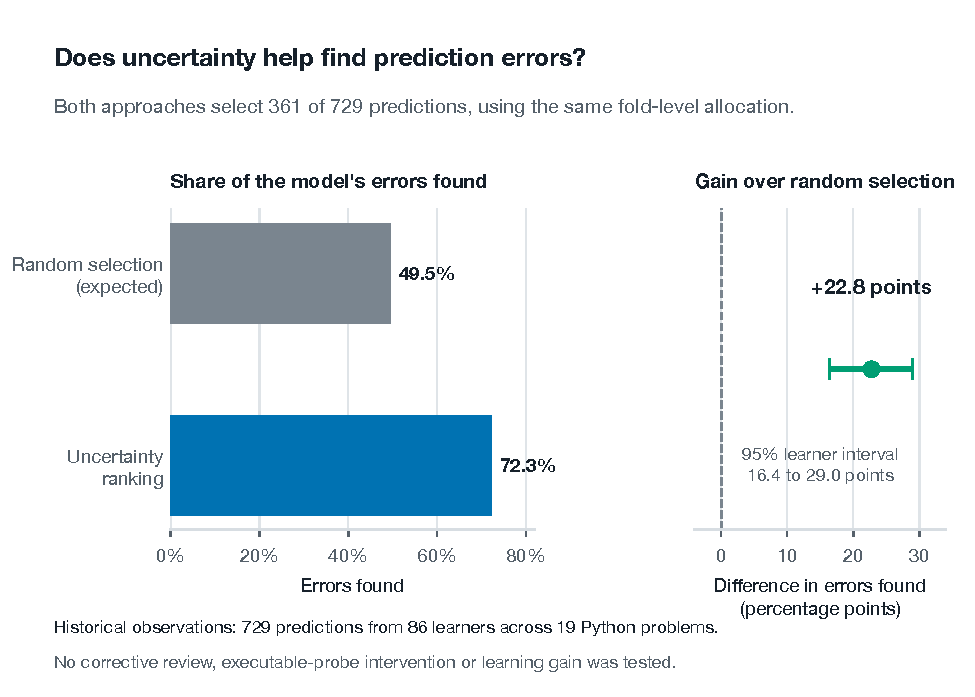
\includegraphics[width=\textwidth]{assets/figures/ch06-evaluation/uncertainty_error_review.pdf}
  \caption{Offline error prioritisation on 729 historical predictions from 86 learners across 19 Python problems. Selecting the
  most uncertain half within each fold, rounded down, captured 141/195 errors across 361 selected predictions. Random selection
  at the same fold allocations would capture 49.5\% in expectation. The gain was 22.8 percentage points (95\% learner bootstrap
  interval: 16.4 to 29.0). Larger values indicate more errors found. The interval conditions on fitted predictions and fixed
  selections. No review intervention, executable probe or learning effect was tested.}
  \label{fig:csedm-result}
\end{figure}

\FloatBarrier
\section{Local Computation and Its Measurement Limits}

The runtime records establish that the simulator work was practical on the development machine. They do not measure a
deployed tutor's response time. The tracker profile used CPython 3.12.13 on macOS with an ARM processor. The acquisition
profile additionally recorded ten logical CPUs and 16 GiB of physical memory. These are development measurements, separate
from the canonical scientific comparisons.

In the tracker timing study, each tracker processed 13,224 recorded updates with available evidence per repetition. An untimed validation pass established a reference checksum, followed by three warm-up repetitions and
twenty timed repetitions. Workload preparation was outside the timed region, and garbage collection was disabled during
measurement. Median time per update ranged from 1.55 microseconds for last-observation tracking to 2.94 microseconds for
bounded channel-aware updating. Ordinary channel-aware updating took 2.73 microseconds. The timed loop included update
invocation and checksum accumulation. These figures describe a prepared workload, not a full tutoring turn or an end-to-end
simulation. No statistical runtime superiority claim follows from them.

The probe selection study's compact development stream was measured in three fresh processes. Each processed 350 episodes across seven settings
and seven policies, producing 98,000 case predictions. Median elapsed time was 4.73 seconds. The largest observed process
peak resident memory was about 78.0 MiB. Timing began after plan loading and included stream generation, serialisation,
hashing and writing to a temporary file, including its final flush to storage. It excluded interpreter startup and downstream
analysis or figure generation. The recorded memory peak includes the process baseline, rather than measuring the policy alone.

Scaling that development time by forty produced a 189-second planning estimate for the canonical workload, or 379 seconds
with the declared factor-of-two allowance. Neither figure is a measured canonical duration. The canonical stream report
records 14,000 episodes, 3,920,000 case predictions across seven policies and 1,960,000 selected simulated probes, with zero
external-model or sandbox calls. These policy-level counts reuse the same episodes. They are not millions of independent
observations. Canonical runtime and peak memory are not recorded in that report and remain unavailable here.

% Sources: tracker development runtime fa5faaff4c604d185cb95486260f1afbceeadc96bd4b291d0dde4c840ce68540;
% acquisition compact runtime 47d0441452375510610b4b2a7e8c1b162e30a5d65896f7177cc9f3e425ec87b5;
% canonical stream cb13c0313c91c11a9cf39c79028180367534357fd6eac4394659e3a819851b60.

\section{What the Uncertainty Intervals Cover}
\suppressfloats[t]

Each interval describes variation under a particular analysis. Table~\ref{tab:interval-scope} states what was resampled
and what remained fixed. Pairing keeps the compared methods on the same cases or episodes. It does not remove limitations
in the data or the generating model.

\begin{table}[htbp]
  \centering
  \caption{Scope of the reported bootstrap intervals. Resampling changes the contribution of observed cases, episodes or
  learners to the estimate. It does not collect new model responses, create new failure settings or retrain the predictors.}
  \label{tab:interval-scope}
  \medskip
  \begin{tabularx}{\textwidth}{@{}>{\raggedright\arraybackslash}p{0.15\textwidth}>{\raggedright\arraybackslash}X>{\raggedright\arraybackslash}X@{}}
    \toprule
    Study & Resampled unit & Fixed inputs and excluded variation \\
    \midrule
    External model & Paired differences for the 23 eligible authored cases. & Recorded model responses, tracker and corrected checks. Case resampling does not account for shared concept families or variability from a new model run. \\
    \addlinespace
    Bounded updates & Paired effects for each episode. Turns are summarised within episodes. & Authored simulator rules and tracker settings. The interval does not describe new failure mechanisms or real learners. \\
    \addlinespace
    Probe selection & Paired episodes within each evaluation environment. Environment means receive equal weight. & Fitted calibration model, policies and six stress settings. Neither calibration refitting nor uncertainty about deployment frequencies is included. \\
    \addlinespace
    Learner records & Learners, keeping each learner's prediction records together. & Fitted predictions from the evaluation folds and selected review cases. Models are not retrained and cases are not ranked again. Dependence from overlapping training folds is not fully represented. \\
    \bottomrule
  \end{tabularx}
\end{table}

Adjusting the three primary probe-selection intervals for multiple comparisons leaves their scope conditional on the fitted
calibration and chosen environments. Development checks of calibration remain diagnostic. The CSEDM intervals likewise
exclude variability from retraining.

More simulated episodes can narrow an interval under the authored rules. They cannot establish that those rules describe
classroom behaviour. The external benchmark, simulations and historical learner analysis therefore retain separate conclusions.

\section{Answers to the Research Questions}

\begin{description}
  \item[RQ1: Extra coding evidence.] The corrected benchmark does not establish whether giving every case an extra coding
  check provides a useful prediction benefit. Accuracy changed from 18 to 19 correct predictions among 23 eligible authored
  cases. The paired interval, 0 to 13.04 percentage points, is too wide to rule in or rule out the declared ten-point useful
  improvement.

  \item[RQ2: Limiting a bad check.] The bounded update passed its prespecified simulator rule. Across the adverse settings,
  its mean Brier error was 0.0094 lower than ordinary channel-aware Bayes, while its clean-setting penalty was 0.0033. Missing
  and contradictory evidence still produced worse individual results, so bounding did not improve every condition.

  \item[RQ3: Choosing checks.] The proposed selector did not choose better cases than all three prespecified comparators at
  the fixed half-budget allocation. It beat random selection by 1.19 percentage points, but its error exceeded
  uncertainty-only selection by 0.86 points and the plug-in clipped-belief rule by 0.54 points. Because its score need not
  equal expected classification-error reduction, this result does not answer whether ordinary value-of-information selection
  would perform better.

  \item[RQ4: Finding likely errors.] In the exploratory CSEDM analysis, uncertainty found more existing prediction errors
  than random selection at the same allocation. It selected 141 of 195 errors, or 72.3\%, compared with 49.5\% expected under
  random selection. No corrective review was performed, so the result does not show that selecting these predictions would
  improve later performance.
\end{description}
